%%%%%%%%%%%%%%%%%%%%%%%%%%%%%%%%%%%%%%%%%%%
%
% From a template maintained at https://github.com/jamesrobertlloyd/cbl-tikz-poster
%
% Code near the top should be fairly standard and not need to be changed
%  - except for the document class
% Code lower down is more likely to be customised
%
%%%%%%%%%%%%%%%%%%%%%%%%%%%%%%%%%%%%%%%%%%%

%%%%%%%%%%%%%%%%%%%%%%%%%%%%%%%%%%%%%%%%%%%
%
% Document class
%
% Change this if you want a different size / orientation poster etc
%
%%%%%%%%%%%%%%%%%%%%%%%%%%%%%%%%%%%%%%%%%%%

\documentclass[landscape,a0b,final,a4resizeable]{a0poster}
%\documentclass[portrait,a0b,final,a4resizeable]{a0poster}

%%%%%%%%%%%%%%%%%%%%%%%%%%%%%%%%%%%%%%%%%%%
%
% 'Basic' packages
%
% TODO - Almost certainly some are unnecessary - feel free to remove nonstandard
% packages if you think it is a good idea not to always have them
%
%%%%%%%%%%%%%%%%%%%%%%%%%%%%%%%%%%%%%%%%%%%

\usepackage{multicol}
\usepackage{color}
\usepackage{shadow}
\usepackage{morefloats}
\usepackage{cite}
\usepackage[pdftex]{graphicx}
\usepackage{rotating}
\usepackage{amsmath, amsthm, amssymb, bm}
\usepackage{array}
\usepackage{nth}
\usepackage[square,numbers]{natbib}
\usepackage{booktabs}

%%%%%%%%%%%%%%%%%%%%%%%%%%%%%%%%%%%%%%%%%%%
%
% TIKZ packages and common definitions
%
% Add extra things as per your tikz needs
%
%%%%%%%%%%%%%%%%%%%%%%%%%%%%%%%%%%%%%%%%%%%

\usepackage{common/picins}
\usepackage{tikz}
\usetikzlibrary{shapes.geometric,arrows,chains,matrix,positioning,scopes,calc}
\tikzstyle{mybox} = [draw=white, rectangle]

%%%%%%%%%%%%%%%%%%%%%%%%%%%%%%%%%%%%%%%%%%%
%
% myfig
%
% \myfig - replacement for \figure
% necessary, since in multicol-environment 
% \figure won't work        
%                 
%%%%%%%%%%%%%%%%%%%%%%%%%%%%%%%%%%%%%%%%%%%

\newcommand{\myfig}[3][0]{
\begin{center}
  \vspace{1.5cm}
  \includegraphics[width=#3\hsize,angle=#1]{#2}
  \nobreak\medskip
\end{center}}

%%%%%%%%%%%%%%%%%%%%%%%%%%%%%%%%%%%%%%%%%%%
%
% mycaption                
%
% \mycaption - replacement for \caption
% necessary, since in multicol-environment \figure and
% therefore \caption won't work
%
%%%%%%%%%%%%%%%%%%%%%%%%%%%%%%%%%%%%%%%%%%%

%\newcounter{figure}
\setcounter{figure}{1}
\newcommand{\mycaption}[1]{
  \vspace{0.5cm}
  \begin{quote}
    {{\sc Figure} \arabic{figure}: #1}
  \end{quote}
  \vspace{1cm}
  \stepcounter{figure}
}

%%%%%%%%%%%%%%%%%%%%%%%%%%%%%%%%%%%%%%%%%%%
%
% Some standard colours
%
%%%%%%%%%%%%%%%%%%%%%%%%%%%%%%%%%%%%%%%%%%%

\definecolor{camlightblue}{rgb}{0.601 , 0.8, 1}
\definecolor{camdarkblue}{rgb}{0, 0.203, 0.402}
\definecolor{camred}{rgb}{1, 0.203, 0}
\definecolor{camyellow}{rgb}{1, 0.8, 0}
\definecolor{lightblue}{rgb}{0, 0, 0.80}
\definecolor{white}{rgb}{1, 1, 1}
\definecolor{whiteblue}{rgb}{0.80, 0.80, 1}

%%%%%%%%%%%%%%%%%%%%%%%%%%%%%%%%%%%%%%%%%%%
%
% Some look and feel definitions
%
%%%%%%%%%%%%%%%%%%%%%%%%%%%%%%%%%%%%%%%%%%%

\setlength{\columnsep}{0.03\textwidth}
\setlength{\columnseprule}{0.0018\textwidth}
\setlength{\parindent}{0.0cm}

%%%%%%%%%%%%%%%%%%%%%%%%%%%%%%%%%%%%%%%%%%%
%
% \mysection - replacement for \section*
% 
% Puts a pretty box around some text
% TODO - any other thoughts for what this box should look like
%
%%%%%%%%%%%%%%%%%%%%%%%%%%%%%%%%%%%%%%%%%%%

\tikzstyle{mysection} = [rectangle, 
									draw=none, 
									shade, 
									outer color=camlightblue!30,
									inner color=camlightblue!30,
									text width=0.965\columnwidth,
									text centered,
									rounded corners=20pt,
									minimum height=0.11\columnwidth]

\newcommand{\mysection}[1]
{
\begin{center}
  \begin{tikzpicture}
    \node[mysection] {\sffamily\bfseries\LARGE#1};
  \end{tikzpicture}
\end{center}
}

%%%%%%%%%%%%%%%%%%%%%%%%%%%%%%%%%%%%%%%%%%%
%
% Set the font
%
% TODO - Not sure what a canonical choice is - feel free to modify
%
%%%%%%%%%%%%%%%%%%%%%%%%%%%%%%%%%%%%%%%%%%%

\renewcommand{\familydefault}{cmss}
\sffamily

%%%%%%%%%%%%%%%%%%%%%%%%%%%%%%%%%%%%%%%%%%%
%
% Poster environment
%
% Centres everything and can be used to define the width of the content
%
%%%%%%%%%%%%%%%%%%%%%%%%%%%%%%%%%%%%%%%%%%%

\newenvironment{poster}{
  \begin{center}
  \begin{minipage}[c]{0.96\textwidth}
}{
  \end{minipage} 
  \end{center}
}

%%%%%%%%%%%%%%%%%%%%%%%%%%%%%%%%%%%%%%%%%%%
%
% This is probably a good place to put content specific packages and definitions
%
%%%%%%%%%%%%%%%%%%%%%%%%%%%%%%%%%%%%%%%%%%%

\newtheorem{thm}{Theorem}%[section]
\newtheorem{lem}[thm]{Lemma}
\newtheorem{prop}[thm]{Proposition}
\newtheorem{cor}[thm]{Corollary}

\newtheorem*{theorem*}{Theorem}

\theoremstyle{definition}
\newtheorem*{definition*}{Definition}
\newtheorem{definition}[thm]{Definition}%[section]
\newtheorem{conj}{Conjecture}[section]
\newtheorem{exmp}{Example}[section]
\newtheorem{rem}[thm]{Remark}

\theoremstyle{remark}
%\newtheorem{rem}{Remark}
\newtheorem{note}{Note}
\newtheorem{case}{Case}

\newcommand{\eqd}{\overset{\,_{\!d}}{=}}
\newcommand{\defn}[1]{\emph{#1}}

\newcommand{\Law}{\mathcal{L}}

\def\given{\,|\,}

\def\SGinf{\mathbb{S}_{\infty}}

\newcommand{\NonNegInts}{\mathbb{Z}_+}
\newcommand{\Nats}{\mathbb{N}}
\newcommand{\Rationals}{\mathbb{Q}}
\newcommand{\Reals}{\mathbb{R}}

\newcommand{\as}{\textrm{a.s.}}

\def\[#1\]{\begin{align}#1\end{align}}
\newcommand{\defas}{:=}

\newcommand{\Normal}{\mathcal{N}}
\newcommand{\dist}{\ \sim\ }

\newcommand{\kernel}{\kappa}
\newcommand{\kernelmatrix}{K}
\newcommand{\scalefactor}{s}
\newcommand{\lengthscale}{\ell}
\newcommand{\targets}{T}
\newcommand{\noise}{\sigma_\targets}
\newcommand{\pseudopoints}{\eta}
\newcommand{\inputpoints}{\xi}
\newcommand{\covhyppar}{\psi}
\newcommand{\logistic}{\phi}

\newcommand{\CompOrder}{\mathcal{O}}
\def\graphspace{\mathbf{G}}
\def\Uniform{\mbox{\rm Uniform}}
\def\Bernoulli{\mbox{\rm Bernoulli}}
\def\ie{i.e.,\ }
\def\eg{e.g.,\ }
\def\iid{i.i.d.\ }
\def\simiid{\sim_{\mbox{\tiny iid}}}
\def\simind{\sim_{\mbox{\tiny ind}}}
\def\eqdist{\stackrel{\mbox{\tiny d}}{=}}
\def\ahfunction{\theta}       
\def\AHfunction{\Theta}           % A-H random function
\def\AHvar{U}                     % A-H uniform variables
\def\AHvaralt{V}                  % A-H uniform variables - for bipartite data
\def\larray{W}                    % latent array sampled with A-H
%\def\latentspace{\mathbf{W}}      % range of entries
\def\latentspace{\mathcal{W}}      % range of entries
\def\darray{X}                    % data array
%\def\dataspace{\mathbf{X}}        % sample space
\def\dataspace{\mathcal{X}}        % sample space
\def\cfspace{\mathbf{C}}          % space of continuous functions
%\def\GP{\mbox{\mathcal{GP}}}
\def\GP{\mathcal{GP}}
\def\likelihood{P}
\def\CovData{C}
\def\CovDataAlt{D}

\def\newarrow{\mbox{\begin{tikzpicture}
             \useasboundingbox{(-3pt,-4.5pt) rectangle (19pt,1pt)};
             \draw[->] (0,-0.07)--(17pt,-0.07);\end{tikzpicture}}}

%%%%%%%%%%%%%%%%%%%%%%%%%%%%%%%%%%%%%%%%%%%
%
% The document environment starts here
%
%%%%%%%%%%%%%%%%%%%%%%%%%%%%%%%%%%%%%%%%%%%

\begin{document}

%%%%%%%%%%%%%%%%%%%%%%%%%%%%%%%%%%%%%%%%%%%
%
% Begin the poster environment - centres things and potentially changes the width
%
%%%%%%%%%%%%%%%%%%%%%%%%%%%%%%%%%%%%%%%%%%%

\begin{poster}

  %%%%%%%%%%%%%%%%%%%%%%%%%%%%%%%%%%%%%%%%%%%
  %
  % Potentially add some space at the top of the poster
  %
  %%%%%%%%%%%%%%%%%%%%%%%%%%%%%%%%%%%%%%%%%%%

  \vspace{0\baselineskip}

  %%%%%%%%%%%%%%%%%%%%%%%%%%%%%%%%%%%%%%%%%%%
  %
  % Draw the header as a TIKZ picture
  %
  % Using TIKZ to allow for easy alignment
  %
  %%%%%%%%%%%%%%%%%%%%%%%%%%%%%%%%%%%%%%%%%%%

  \begin{center}
    \begin{tikzpicture}[x=0.5\textwidth]
      % Dummy nodes at edges for spacing
      % TODO - a better way?
      \node at (+1, 0) {};
      \node at (-1, 0) {};
      % Set the size of the badges
      \def \badgeheight {0.08\textwidth}
      % Title text
      \node[inner sep=0,text width=0.75\textwidth,text centered,font=\Huge] (Title) at (0,0)
      {
      {\sffamily \Huge \textbf{Personalized Recipe Recommendation Using Heterogeneous Graphs}}\\
      {\huge\sffamily
      Nicholas B. DeGroot\textsuperscript{1},
      Jonathan Herke\textsuperscript{2},
      Jay Yu\textsuperscript{2}
      }\\
      \vspace{-0.3\baselineskip}
      {\large\sffamily
        1: HDSI, University of California San Diego, USA
        2: TigerGraph, USA
      }
      };
      % UCSD badge
      \node [mybox] (UCSD Badge) at (-0.9, 0) {
        
\includegraphics[height=\badgeheight]{badges/ucsdseal.png}
      };
      % TigerGraph badge
      \node [mybox] (TigerGraph Badge) at (0.9, 0) {
        
\includegraphics[height=\badgeheight]{badges/tigergraph.png}
      };
    \end{tikzpicture}
  \end{center}
  %%%%%%%%%%%%%%%%%%%%%%%%%%%%%%%%%%%%%%%%%%%
  %
  % Spacing between title and main body
  %
  %%%%%%%%%%%%%%%%%%%%%%%%%%%%%%%%%%%%%%%%%%%

  \vspace{1\baselineskip}

  %%%%%%%%%%%%%%%%%%%%%%%%%%%%%%%%%%%%%%%%%%%
  %
  % Columns environment
  %
  %%%%%%%%%%%%%%%%%%%%%%%%%%%%%%%%%%%%%%%%%%%

  \begin{multicols}{3}

    %%%%%%%%%%%%%%%%%%%%%%%%%%%%%%%%%%%%%%%%%%%
    %
    % Start of content
    %
    %%%%%%%%%%%%%%%%%%%%%%%%%%%%%%%%%%%%%%%%%%%

    \large

    \mysection{Abstract}

    \begin{itemize}
      \item TODO
    \end{itemize}

    \vspace{\baselineskip}
    \mysection{Motivation}

    \begin{center}
      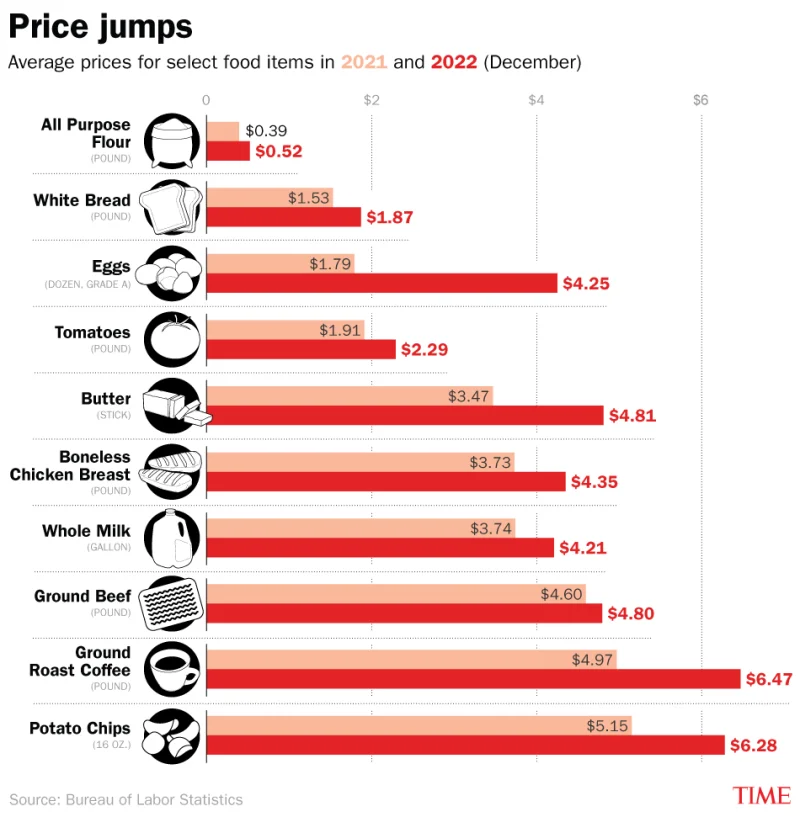
\includegraphics[height=9.5\baselineskip]{figures/food-inflation.png}
      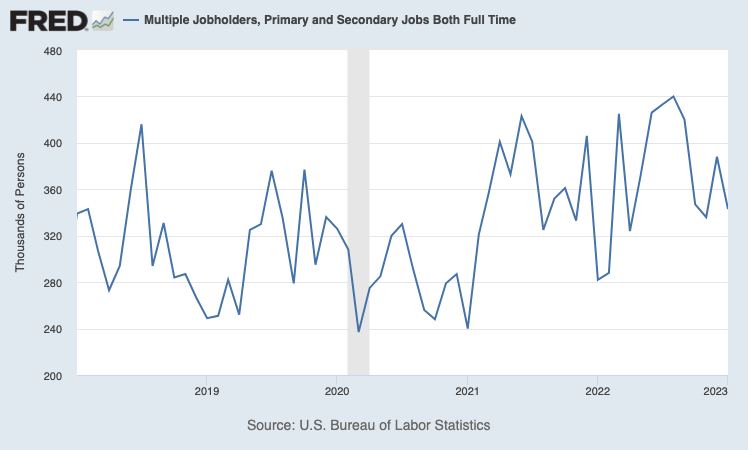
\includegraphics[height=9.5\baselineskip]{figures/two-jobs.png}
    \end{center}

    \textbf{TA Note:} I plan on pulling the data and creating graphs more stylistically in-line with the project.

    \vspace{\baselineskip}

    This project was born from some recent insights in the economy:
    \begin{itemize}
      \item Roughly 388,000 Americans are currently working more than two \textbf{full time} jobs (nearly 5\% of the workforce).
      \item The average cost of groceries for a household has risen by 13.5\% over the last year.
    \end{itemize}

    In essence, people can't afford to eat out due to budget constraints, but can't afford to eat at home due to time constraints. To this end, we propose a system that can automate the process of meal planning and grocery shopping. By automatically generating meal plans custom tailored to the users taste preferences, users save the time previously spent planning meals and the money previously spent eating out.

    \vspace{\baselineskip}
    \mysection{Collaborative Filtering}

    The obvious solution to this problem is with \textit{collaborative filtering}. Collaborative filtering works by finding users with similar tastes and recommending items that those users have liked.

    We chose to define similarity as the pearson correlation between user's reviews, with the rating being equivalent to an edge weight.

    $$
      Sim(u, o) = \frac
      {
        \sum_{i \in I_u \cup I_o} (R_{u,i} - \bar{R_u})(R_{o,i} - \bar{R_o})
      }{
        \sqrt{
          \sum_{i \in I_u \cup I_o} (R_{u,i} - \bar{R_u})^2
          \sum_{i \in I_u \cup I_o} (R_{o,i} - \bar{R_o})^2
        }
      }
    $$

    \vspace{\baselineskip}
    This approach has a number of advantages:
    \begin{itemize}
      \item Cheap calculation (particularly in a Graph DB)
      \item Explainable / understandable
    \end{itemize}

    \vspace{\baselineskip}
    But doesn't come without its drawbacks:
    \begin{itemize}
      \item Ignores extra recipe information
      \item Ignores higher-order relationships (i.e. ingredients)
    \end{itemize}

    \newpage
    \mysection{Expanding with LightGCN}

    We can fix a number of these drawbacks by drawing on the power of graph neural networks. By extending the work of \citet{lightgcn}, we can use a graph neural network to learn latent features for both users and recipes, and use them to make recommendations.

    \vspace{\baselineskip}
    The model can be summarized as such:
    \begin{itemize}
      \item Goal: Learn latent features for users and recipes. Users with a high affinity for a recipe should have a high latent feature similarity (defined by cosine similarity).
      \item Each iteration, the model updates the latent features of each user and recipe by taking a weighted average of the latent features of their neighbors.
            $$
              \mathbf{x}_i = \sum_{j \in \mathcal{N}(i)}
              \frac{1}{\sqrt{\deg(i)\deg(j)}}\mathbf{x}^{(l)}_j
            $$
      \item Loss: Bayesian Personalized Ranking loss (BPR). Given a positive ($+$) and negative ($-$) user-recipe interaction:
            $$
              \mathcal{L} = -\frac{1}{N}\sum_{(u, +, -) \in \mathcal{D}}
              \log\sigma(\mathbf{x}_+ - \mathbf{x}_-)
            $$
    \end{itemize}

    We can further improve the performance in two ways:
    \begin{itemize}
      \item Concatenating known recipe information (e.g. nutritional information, cooking time, etc.) with the learned latent features.
      \item Weighing the edges of each recipe with the review score.
    \end{itemize}

    \vspace{\baselineskip}
    \mysection{Higher-Order Relationships}

    While an improvement over baseline collaborative filtering, LightGCN still ignores higher-order relations such as shared ingredients and user-generated tags.

    TODO.

    \newpage
    \mysection{Comparison of Methods}

    TODO


    \vspace{\baselineskip}
    \mysection{Conclusion}
    TODO

    \vspace{\baselineskip}
    \bibliographystyle{dinat}
    \bibliography{citations}

    \vspace{\baselineskip}
    \begin{tabular}{cc}
      \begin{minipage}[c]{0.8\columnwidth}

        Code at \texttt{github.com/nickthegroot/recipe-recommendation}

        Paper available by scanning the QR code

      \end{minipage}
       &
      \begin{minipage}[c]{0.2\columnwidth}
        \begin{centering}
          
\includegraphics[width=\linewidth]{figures/report_qr.png}
        \end{centering}
      \end{minipage}
    \end{tabular}

  \end{multicols}

\end{poster}

\end{document}
